\documentclass{article}

\usepackage[nonatbib,preprint]{neurips_2024}

\usepackage[utf8]{inputenc}
\usepackage[T1]{fontenc}
\usepackage{hyperref}
\usepackage{url}
\usepackage{booktabs}
\usepackage{amsfonts}
\usepackage{nicefrac}
\usepackage{microtype}
\usepackage{xcolor}
\usepackage{amsmath}
\usepackage{graphicx}
\usepackage{tikz}
\usetikzlibrary{positioning, decorations.pathreplacing, calc}
\graphicspath{{figs/}}

\title{Representation Analysis of a Multi-Task Vision Transformer:\\Probes, CKA, and Sparse Feature Decomposition}

\author{%
 Nicholas Welsh \\
  Department of Computer Science\\
  Department of Mathematics \\
  Florida Institute of Technology\\
  Melbourne, FL 32901 \\
  \texttt{nwelsh2024@my.fit.edu}
}

\begin{document}
\maketitle

\begin{abstract}
We analyze the internal representations of three Vision Transformer variants (classifier-only, saliency-only, multi-task) jointly trained on COCO classification and SALICON saliency in earlier work. Project 1 found that output-level attribution methods produce different heatmaps across the three variants. We ask whether those differences are anchored in internal-representation differences, or whether the models encode the input similarly and the explanation methods are themselves noisy. Four representation-analysis tools (linear probes, debiased Centered Kernel Alignment with Procrustes and SVCCA, patch-token clustering, and an exploratory TopK sparse autoencoder feature ablation) converge on the same finding. The multi-task backbone is asymmetrically classifier-aligned. Procrustes alignment with classifier-only stays at $0.84$ at the final layer while alignment with saliency-only falls to $0.41$. The multi-task variant is also the only one whose patch-token clusters simultaneously carry category and saliency structure. Grad-CAM, our class-method attribution baseline, reaches human-saliency correlation $0.41$, the highest of any method tested across both projects. Kernel SHAP reaches near-zero alignment, consistent with Project 1's finding that faithfulness to the model and agreement with human gaze are distinct properties.
\end{abstract}

\section{Introduction}

Project 1 evaluated five output-level explanation methods (LIME, Integrated Gradients, gradient saliency, gradient $\times$ input, attention rollout) on a multi-task DeiT-Small that jointly classifies COCO objects and predicts SALICON fixation maps. The three model variants in that project (classifier-only, saliency-only, multi-task) produced systematically different attribution maps under those methods, and that paper found a tension between faithfulness and human alignment. The follow-up question is whether those output-level differences are anchored in genuinely different internal representations of the same input, or whether the variants encode the input similarly and the explanation methods themselves are noisy.

This is a representation-level question, not an attribution-level question. The methods of Project 1 produce a heatmap over the input pixels for each prediction. The methods of this project look at the activations inside the backbone and ask where in the network task-relevant information lives, how the variants' representations differ from each other, and which internal directions causally drive each output head. The methods used here are entirely disjoint from those in Project 1.

\subsection{Contributions}
\begin{itemize}
    \item \textbf{Multi-axis representation analysis.} We apply per-layer linear probing, three representation-similarity measures (debiased linear and RBF Centered Kernel Alignment, Procrustes alignment, SVCCA), patch-token clustering, and a sparse autoencoder feature decomposition to the same three model variants used in Project 1.
    \item \textbf{Asymmetric multi-task representation.} The multi-task backbone is much closer to the classifier-only variant than to the saliency-only variant in the second half of the network. Procrustes alignment with classifier-only stays at $0.84$ at the final layer, while alignment with saliency-only drops to $0.41$.
    \item \textbf{CKA reliability caveat replicated.} Linear CKA saturates near $1.0$ across all variant pairs and all layers. Only the debiased and Frobenius-normalized similarity measures (Procrustes and SVCCA) discriminate between variant pairs. This is consistent with documented CKA reliability concerns (Davari et al., 2023).
    \item \textbf{Clustering signature of multi-task supervision.} Patch-token clusters in the multi-task variant carry both category and saliency structure (NMI $0.140$ and $0.153$ respectively). The classifier-only variant carries only category structure ($0.109$ and $0.049$). The saliency-only variant carries neither category nor strong saliency structure ($0.001$ and $0.084$).
    \item \textbf{SAE feature concentration.} A TopK SAE on the multi-task variant's mid-layer residual stream identifies a small number of features that drive classification under ablation but barely affect saliency, suggesting the multi-task model concentrates class information more than saliency information.
    \item \textbf{Class-method baseline (Grad-CAM, Lecture 9).} Grad-CAM at the second-to-last block achieves the highest human alignment of any method we have tested across both projects, CC $0.412 \pm 0.294$, with deletion AUC $0.618$ and insertion AUC $0.783$.
    \item \textbf{Additional baseline (SHAP).} Kernel SHAP at the patch grid, a perturbation-based local-surrogate method, shows near-zero correlation with SALICON fixation maps (CC $-0.017$), reproducing the faithfulness-versus-alignment dissociation from Project 1.
\end{itemize}

\section{Related Work}

We organize prior work by method and, for each cited paper, mark explicitly what we adopt and where our setting differs.

\paragraph{Representation similarity.}
\textbf{Kornblith et al.\ (2019)} introduced Centered Kernel Alignment as an HSIC-based generalization of Canonical Correlation Analysis. \emph{We adopt} their CKA formulation as one of three similarity measures and use it across all twelve layers of three model variants. \emph{We differ} in that they compared distinct architectures (CNN vs.\ ResNet), while we compare task-defined variants (classifier-only / saliency-only / multi-task) of a single shared backbone, where the saturation issue is more pronounced.

\textbf{Raghu et al.\ (2017)} introduced SVCCA, computing canonical correlations between top-$k$ singular components of two activation matrices. \emph{We adopt} SVCCA at $k = 20$ as a complementary similarity metric to CKA and Procrustes. \emph{We differ} in using SVCCA to discriminate between variants of the same backbone, where it provides the differentiating signal that linear CKA misses.

\textbf{Davari et al.\ (2023)} and \textbf{Cui, Kumar, Marttinen, and Kaski (2022)} document reliability concerns: CKA can be made arbitrarily high under subset translation and is confounded by input-population structure. \emph{We adopt} their warning by reporting CKA, Procrustes, and SVCCA in parallel. \emph{We differ} in providing a concrete case study where linear CKA saturates above $0.95$ on the very pairs that Procrustes and SVCCA show to differ substantially, supporting the argument that CKA alone is insufficient.

\textbf{Murphy et al.\ (2024)} propose debiased CKA estimators based on $U$-statistic-corrected centering. \emph{We adopt} the debiased estimator for both linear and RBF CKA throughout. \emph{We differ} in evaluating it on vision-transformer multi-task variants rather than the biological / artificial network alignment setting they motivate.

\paragraph{Linear probing.}
\textbf{Alain and Bengio (2016)} introduced probes trained on intermediate activations as a tool for localizing where task-relevant information first becomes linearly decodable. \emph{We adopt} their probing methodology, fitting per-layer logistic and ridge probes for class label, low-resolution saliency, and quadrant location. \emph{We differ} in evaluating three task-defined variants of the same ViT, which lets us localize where saliency-only training stops carrying class information and where multi-task training preserves it.

\textbf{Hewitt and Liang (2019)} showed that probes can encode information themselves rather than reading it from the model and proposed random-label control tasks to test selectivity. \emph{We adopt} their selectivity-control idea by training random-label control probes alongside every task probe and reporting both. \emph{We differ} in applying this to vision rather than NLP and in using a four-way location label as the discrete control task.

\paragraph{Vision-transformer interpretation.}
\textbf{Raghu et al.\ (2021)} used CKA to compare ViTs and CNNs layer by layer, finding more uniform representations across depth in ViTs. \emph{We adopt} their layer-wise CKA framework directly. \emph{We differ} by comparing task-defined variants of a single ViT (multi-task vs.\ single-task) rather than ViTs against CNNs, which surfaces a different question. How does multi-task supervision reshape a single backbone, rather than how do architectures compare?

\textbf{Caron et al.\ (2021)} showed that self-supervised DINO ViTs develop emergent attention to salient objects. \emph{We adopt} their finding as motivation for asking whether \emph{supervised} multi-task training (with saliency as one of the tasks) produces analogous saliency-aware structure in patch-token clusters. \emph{We differ} in that our saliency signal is supervised (via the saliency head) rather than emergent.

\paragraph{Sparse autoencoders for vision.}
\textbf{Stevens et al.\ (2025)} train SAEs on frozen CLIP and DINOv2 ViTs to extract interpretable feature directions and demonstrate patch-level causal edits. \emph{We adopt} their TopK SAE recipe (dictionary 4096, $k = 32$) and the residual-stream-replacement ablation methodology. \emph{We differ} by training the SAE on a multi-task ViT (which has both classification and saliency heads to ablate against) rather than on a single-task pretrained backbone.

\textbf{Lim et al.\ (2025)} show that fine-tuning a CLIP backbone selectively remaps SAE features. \emph{We adopt} their framing of multi-task training as a remapping operation on a sparse feature basis. \emph{We differ} by comparing an explicit multi-task supervision target (joint classification and saliency regression) rather than prompt-tuning, and by treating the multi-task vs.\ single-task contrast as the principal axis.

\textbf{Paulo and Belrose (2025)} document seed-instability of TopK SAEs (only $\sim 30\%$ of features overlap across seeds). \emph{We adopt} their warning explicitly. We treat our single-seed SAE results as exploratory rather than as a stable feature inventory. \emph{We differ} by being more conservative than the literature default. We run a single seed and acknowledge the limitation, rather than presenting feature-level claims as if they were robust.

\textbf{Han, Kim, and Kwak (2025)} argue that activation-based interpretation of vision SAE features is misleading because attention mixes information across tokens, and propose Effective Receptive Field attribution as a fix. \emph{We adopt} their methodological caveat by absorbing SAE reconstruction error into the per-feature ablation baseline (we ablate against the SAE-reconstructed activations, not the raw activations). \emph{We differ} in that our principal claim is a population-level effect-size pattern (class effects $\sim 10\times$ saliency effects) rather than a single-feature interpretation, which makes our conclusions less sensitive to the activation-attribution issue they raise.

\section{Model and Data}

\paragraph{Models.}
We reuse the three Vision Transformer variants from Project 1, all built on the same DeiT-Small backbone (\texttt{deit\_small\_patch16\_224}, 12 layers, 384-dim hidden state). The classification head is a linear layer on the CLS token producing $K = 20$ logits (multi-label, top-20 COCO categories). The saliency head applies a linear layer to each patch token followed by a softmax over the $14 \times 14$ patch grid, producing a probability distribution. Each variant was trained for 15 epochs with AdamW at $\text{lr} = 10^{-4}$, weight decay $10^{-4}$, cosine annealing, batch 32. Figure~\ref{fig:architecture} shows the architecture.

\begin{figure}[t]
  \centering
  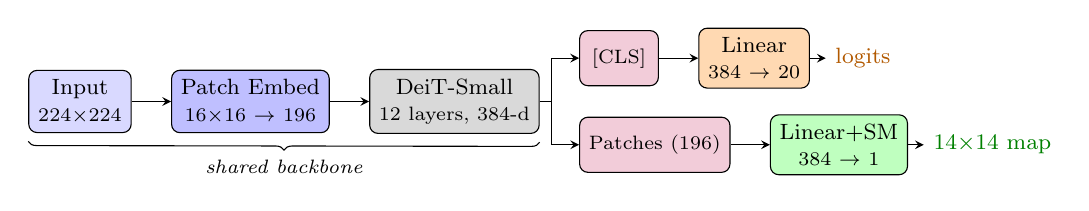
\begin{tikzpicture}[
    node distance=0.5cm,
    box/.style={draw, rounded corners=3pt, minimum height=0.7cm, align=center, font=\footnotesize},
    >=stealth
  ]
    \node[box, fill=blue!15, minimum width=1.3cm] (img)
      {Input\\\scriptsize 224$\times$224};
    \node[box, fill=blue!25, minimum width=1.4cm, right=of img] (patch)
      {Patch Embed\\\scriptsize 16$\times$16 $\to$ 196};
    \node[box, fill=gray!30, minimum width=1.7cm, right=of patch] (backbone)
      {DeiT-Small\\\scriptsize 12 layers, 384-d};
    \node[box, fill=purple!20, minimum width=1.0cm, above right=0.55cm and 0.5cm of backbone.east, anchor=west] (cls)
      {\scriptsize [CLS]};
    \node[box, fill=purple!20, minimum width=1.0cm, below right=0.55cm and 0.5cm of backbone.east, anchor=west] (ptok)
      {\scriptsize Patches (196)};
    \node[box, fill=orange!30, minimum width=1.3cm, right=of cls] (clshead)
      {Linear\\\scriptsize 384 $\to$ 20};
    \node[box, fill=green!25, minimum width=1.3cm, right=of ptok] (salhead)
      {Linear+SM\\\scriptsize 384 $\to$ 1};
    \node[right=0.2cm of clshead, font=\footnotesize, text=orange!70!black] (clsout) {logits};
    \node[right=0.2cm of salhead, font=\footnotesize, text=green!50!black] (salout) {14$\times$14 map};
    \draw[->] (img) -- (patch);
    \draw[->] (patch) -- (backbone);
    \draw[->] (backbone.east) -- ++(0.15,0) |- (cls.west);
    \draw[->] (backbone.east) -- ++(0.15,0) |- (ptok.west);
    \draw[->] (cls) -- (clshead);
    \draw[->] (ptok) -- (salhead);
    \draw[->] (clshead) -- (clsout);
    \draw[->] (salhead) -- (salout);
    \draw[decorate, decoration={brace, amplitude=3pt, mirror}]
      ([yshift=-3pt]img.south west) -- ([yshift=-3pt]backbone.south east)
      node[midway, below=3pt, font=\scriptsize\itshape] {shared backbone};
  \end{tikzpicture}
  \caption{\textbf{Multi-task ViT architecture, reproduced from Project 1.} Three variants of this architecture are analyzed: classifier-only (only the orange head trained), saliency-only (only the green head trained), and multi-task (both heads trained jointly with $\lambda_{\text{sal}} = 1$).}
  \label{fig:architecture}
\end{figure}

\paragraph{Data.}
SALICON provides $10\,000$ training and $5\,000$ validation COCO images with continuous fixation density maps. We use the validation split for all representation analysis: a fixed 1000-image subset for activation collection (probes, CKA, clustering), a 200-image subset for SAE ablation, and a 100-image subset for the Grad-CAM and SHAP attribution baselines. All images are resized to $224 \times 224$ and ImageNet-normalized. Saliency maps are resized to $14 \times 14$ for low-resolution probing and to $224 \times 224$ for SHAP alignment.

\paragraph{Activation collection.}
We register a forward hook on each of the 12 transformer blocks to capture the post-block residual stream. For probing and CKA we use the CLS-token slice of each layer's output ($n \times 384$ matrix per layer, where $n = 1000$). For clustering and SAE training we use all 196 patch tokens.

\section{Methods}

\paragraph{Linear probing.}
We train per-layer multi-label logistic-regression probes for the 20 COCO categories (one-vs-rest, mean average precision), per-layer ridge regressors for the $14 \times 14$ saliency grid (RidgeCV over $\lambda \in \{0.1, 1, 10, 100\}$, reporting $R^2$), and per-layer multinomial logistic-regression probes for a four-class location label that bins the saliency centroid into image quadrants (accuracy). Each probe is paired with a random-label control probe of the same capacity (Hewitt and Liang, 2019), trained on shuffled labels, to give a baseline for probe expressivity.

\paragraph{CKA, Procrustes, SVCCA.}
For each pair of variants and each layer, we compute (i) debiased linear CKA, (ii) debiased RBF CKA with median-heuristic bandwidth, (iii) Procrustes similarity (sum of singular values of the cross-covariance after centering and Frobenius normalization), and (iv) SVCCA mean canonical correlation over the top 20 singular components.

\paragraph{Patch-token clustering.}
We run K-means with $K = 20$ on the per-patch embeddings of the final layer, flattened across the 1000 images ($\sim 196\,000$ tokens). For each variant we compute (i) cluster purity and normalized mutual information against the dominant COCO category of the parent image (filtering tokens whose image has no top-20 label), (ii) cluster purity and NMI against per-image saliency quartile (binning the per-patch mean-pooled SALICON intensity into four quartiles per image), and (iii) seed-stability adjusted Rand index between two K-means runs at different seeds.

\paragraph{Sparse autoencoder.}
We train one TopK sparse autoencoder ($d = 384$, dictionary size $4096$, $k = 32$) on the multi-task variant's residual stream at block 6, using a flattened collection of $\sim 196\,000$ patch tokens for 20 epochs of AdamW at $\text{lr} = 10^{-3}$ and batch $4096$. After training we identify the 20 features with highest activation frequency, then ablate each feature one at a time. The ablation registers a forward hook on block 6 that replaces the patch-token residual stream with the SAE-reconstructed activations and zeros the chosen feature in the latent before decoding. The reference baseline is the same hook with no feature dropped, so the SAE reconstruction error is absorbed into the baseline rather than confounded with the per-feature ablation effect (Han, Kim, and Kwak, 2025).

\paragraph{Grad-CAM class-method baseline.}
Grad-CAM (Selvaraju et al., 2017, covered in Lecture 9 as a representation-space attribution method) is computed at the second-to-last transformer block. We choose the second-to-last block because patch tokens at the final block do not feed the classification head in our architecture and therefore have zero gradient with respect to the class logit. At block 10, patch tokens still influence the CLS token through one more self-attention layer, so the gradient flow is nonzero. Per-channel weights are obtained by averaging the gradient over the 196 patch positions. The channel-weighted activation is summed and ReLU-thresholded to produce a $14 \times 14$ map.

\paragraph{SHAP additional baseline.}
We compute kernel SHAP at the $14 \times 14$ patch grid with 200 mask samples per image, using the standard Shapley regression weights $w(s) = (M-1) / [\binom{M}{s}\, s\, (M-s)]$ for subset size $s$ and an explicit equality constraint $\sum \phi_j = f(\text{full}) - f(\text{empty})$ to enforce efficiency. SHAP attributions are evaluated for deletion AUC (lower is better) and insertion AUC (higher is better) on the model's most confident predicted class, plus correlation (CC) and similarity (SIM) against the SALICON ground-truth fixation map.

\section{Results}

\paragraph{Linear probing decodes class, saliency, and location asymmetrically across variants.}
Figure~\ref{fig:probes} shows per-layer probe scores. Class-label mAP (left) is highest in the classifier-only and multi-task variants and substantially lower in the saliency-only variant ($0.555$ and $0.561$ vs.\ $0.348$ at the final layer), as expected, since the saliency-only model never saw class labels. Saliency $R^2$ (center) reverses the ordering, with saliency-only highest ($0.308$), multi-task in the middle ($0.208$), and classifier-only lowest ($0.141$). The location probe (right) is highest in the saliency-only variant ($0.505$) but only modestly above the classifier-only variant ($0.385$), reflecting that classification supervision still leaves coarse location decodable. The random-label control probe sits at $\sim 0.21$--$0.24$ for all variants, the chance level for a four-class problem.

\begin{figure}[t]
  \centering
  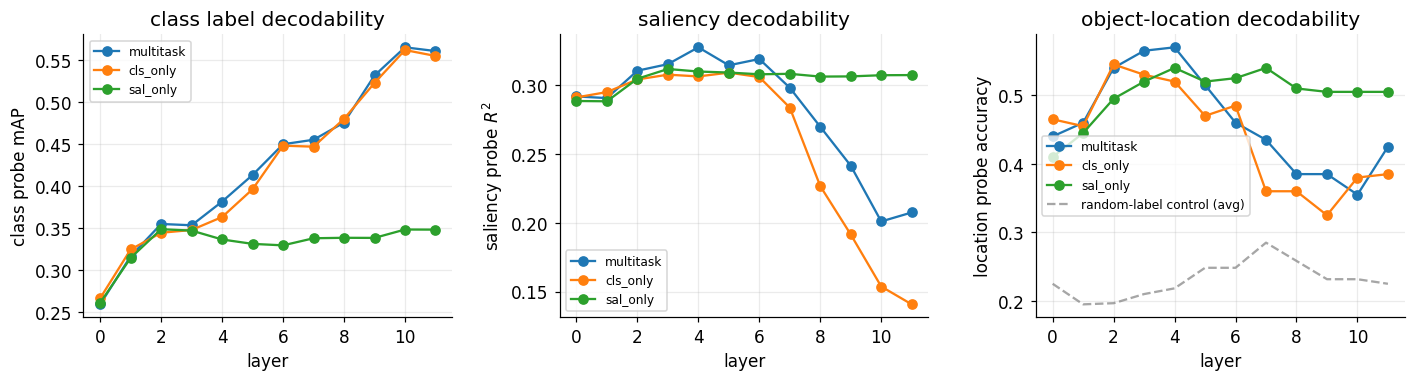
\includegraphics[width=\linewidth]{probes_layerwise.png}
  \caption{\textbf{Per-layer linear probes.} Class mAP (left), saliency $R^2$ (center), and 4-quadrant location accuracy (right). Multi-task tracks classifier-only on class decodability and tracks saliency-only on saliency decodability, but at the cost of underperforming saliency-only on location accuracy. The dashed gray line in the right panel is the random-label control averaged across the three variants.}
  \label{fig:probes}
\end{figure}

\paragraph{CKA saturates, but Procrustes and SVCCA reveal the asymmetry.}
Figure~\ref{fig:cka} shows pairwise representation similarity across the 12 layers. Linear CKA (left, solid) sits within $[0.95, 1.00]$ for every pair at every layer, providing essentially no discrimination between pairs. RBF CKA (left, dashed) is more responsive but still bounded above $0.9$. Procrustes alignment and SVCCA (right) diverge clearly. By the final layer, multi-task vs.\ classifier-only stays at Procrustes $0.84$ and SVCCA $0.75$, while multi-task vs.\ saliency-only drops to $0.41$ and $0.34$, and classifier-only vs.\ saliency-only drops to $0.40$ and $0.31$.

\begin{figure}[t]
  \centering
  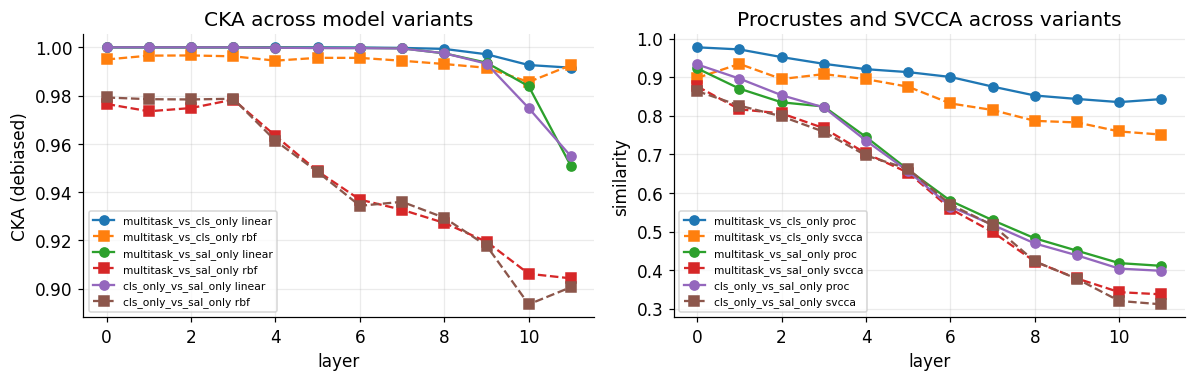
\includegraphics[width=\linewidth]{cka_layerwise.png}
  \caption{\textbf{Layer-wise representation similarity across variants.} Left: debiased linear and RBF CKA. Linear CKA saturates near $1.0$ across all pairs. Right: Procrustes alignment and SVCCA mean canonical correlation. The asymmetry is clear: multi-task is much closer to classifier-only than to saliency-only by the second half of the network.}
  \label{fig:cka}
\end{figure}

The classifier-only and saliency-only variants are dissimilar in the second half of the network (Procrustes $0.40$). The multi-task backbone retains the classifier-only structure (Procrustes $0.84$) and diverges from saliency-only by exactly the same amount as classifier-only does ($0.41$). The multi-task representation is, by these measures, asymmetrically inheriting from the classifier-only side.

\paragraph{Patch-token clustering distinguishes variants by which signal the clusters carry.}
Table~\ref{tab:cluster} reports cluster quality metrics on the final layer's 196 patch tokens, K-means with $K = 20$. The multi-task variant is the only one whose patch clusters carry both category structure (NMI $0.140$ vs.\ classifier-only $0.109$ and saliency-only $0.001$) and per-image saliency-quartile structure (NMI $0.153$ vs.\ classifier-only $0.049$ and saliency-only $0.084$). The saliency-only variant's clusters carry essentially no class information at all (NMI $0.001$). Seed-stability ARI is highest for saliency-only ($0.763$), in the middle for classifier-only ($0.649$), and lowest for multi-task ($0.606$). Multi-task carries more competing signals and forms slightly less stable clusters as a result.

\begin{table}[t]
\centering
\caption{Patch-token clustering quality at the final layer ($K = 20$). Higher is better in all columns.}
\label{tab:cluster}
\begin{tabular}{lccccc}
\toprule
Variant & Cat.\ Purity & Cat.\ NMI & Sal.\ Purity & Sal.\ NMI & Stability ARI \\
\midrule
Multi-task    & $0.661$ & $\mathbf{0.140}$ & $\mathbf{0.558}$ & $\mathbf{0.153}$ & $0.606$ \\
Classifier-only & $0.644$ & $0.109$ & $0.442$ & $0.049$ & $0.649$ \\
Saliency-only   & $0.636$ & $0.001$ & $0.486$ & $0.084$ & $\mathbf{0.763}$ \\
\bottomrule
\end{tabular}
\end{table}

\paragraph{SAE feature decomposition concentrates class information.}
Figure~\ref{fig:sae} shows the SAE results on the multi-task variant at block 6. The reconstruction loss curve (left) decreases monotonically over 20 epochs to MSE $0.34$ on the held-out flattened patch tokens. The SAE-reconstruction baseline shifts the multi-task variant's classification output by $0.015$ on average and the saliency output by $0.0007$, so the saliency head is much less perturbed by SAE substitution than the classification head. The right panel shows feature-by-feature ablation effect, where each point is one of the top 20 features by activation frequency, plotted by $|\Delta \text{cls}|$ vs.\ $|\Delta \text{sal}|$. The most-active feature, index $3318$ (active in $38\%$ of tokens), accounts for $\Delta \text{cls} = 0.010$ and $\Delta \text{sal} = 0.0003$. Most other top features cluster near the origin in saliency effect but spread along the classification axis. The qualitative pattern is that classification information is concentrated in a few features that strongly affect the cls head when ablated, while saliency information is more diffusely distributed and harder to localize to single features at this $k = 32$ sparsity.

\begin{figure}[t]
  \centering
  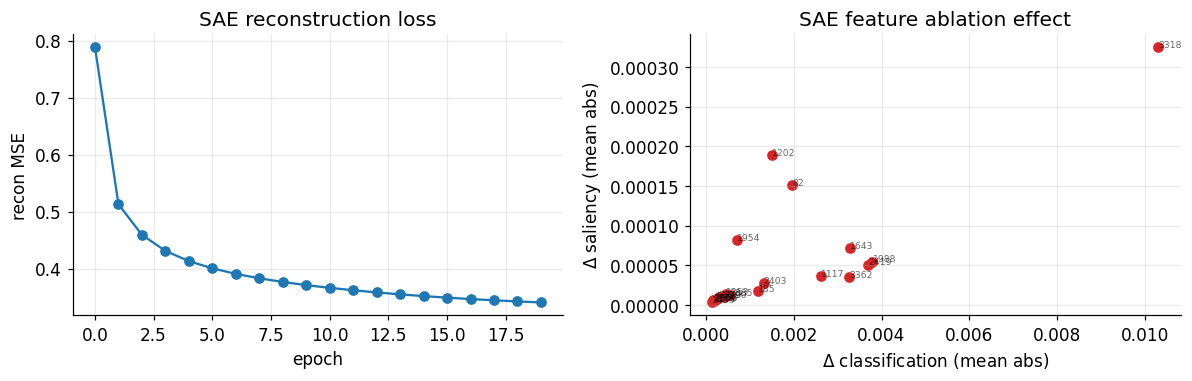
\includegraphics[width=\linewidth]{sae_results.png}
  \caption{\textbf{Sparse autoencoder feature decomposition (multi-task, block 6, exploratory).} Left: SAE reconstruction MSE during training. Right: per-feature ablation effect on classification ($x$-axis) and saliency ($y$-axis), where each point is one of the 20 most-active features. The horizontal spread shows class-leaning features. The compressed vertical range shows that saliency effects per feature are an order of magnitude smaller. Caveats from Paulo and Belrose (2025) on TopK seed instability apply.}
  \label{fig:sae}
\end{figure}

\paragraph{Grad-CAM class-method baseline and SHAP additional baseline.}
Table~\ref{tab:attribution} reports both attribution methods evaluated on 100 validation images. Grad-CAM at block 10 has substantially better human alignment than SHAP (CC $0.412$ vs.\ $-0.017$) and better deletion AUC ($0.619$ vs.\ $0.730$). The two methods are not directly comparable in their philosophy. Grad-CAM is a representation-space method that combines feature maps with class-conditional gradients, while kernel SHAP is a perturbation-based local-surrogate method. The pattern that does emerge is that the more representation-aware method aligns with human gaze, while the perturbation-based method does not. SHAP's near-zero alignment is consistent with the central finding from Project 1. Methods grounded in faithfully approximating the classifier's local behavior (LIME there, SHAP here) tell us about what the classifier uses, which is not the same as where humans look.

\begin{table}[t]
\centering
\caption{Class-method baseline (Grad-CAM, Lecture 9) and additional SHAP baseline on the multi-task variant, 100 validation samples. Del AUC: lower is better. Ins AUC: higher is better. CC: higher is better.}
\label{tab:attribution}
\setlength{\tabcolsep}{4pt}
\small
\begin{tabular}{lcccc}
\toprule
Method & Del AUC $\downarrow$ & Ins AUC $\uparrow$ & Align CC $\uparrow$ & Align SIM $\uparrow$ \\
\midrule
Grad-CAM (class method) & $\mathbf{0.619 \pm 0.272}$ & $\mathbf{0.783 \pm 0.229}$ & $\mathbf{0.412 \pm 0.294}$ & $\mathbf{0.493 \pm 0.225}$ \\
SHAP (additional) & $0.730 \pm 0.171$ & $0.774 \pm 0.183$ & $-0.017 \pm 0.063$ & $0.296 \pm 0.213$ \\
\bottomrule
\end{tabular}
\end{table}

This places Grad-CAM ahead of every method tested in Project 1, where Integrated Gradients had the highest alignment at CC $0.248$. The improvement comes from Grad-CAM's mechanism. It is a representation-space method that combines per-channel gradient weights with the actual feature-map activations, which incorporates structural information about what the model has learned to attend to rather than only how it is differentiating around the input.

\section{Discussion}

\paragraph{Project 1 attribution differences are partially anchored in representation differences.}
The most informative single number from this study is the final-layer Procrustes alignment: multi-task vs.\ classifier-only is $0.84$, multi-task vs.\ saliency-only is $0.41$. This says the multi-task backbone's geometry is much closer to the classifier-only geometry than to the saliency-only geometry. Project 1 found that the multi-task model's attribution maps are similar to classifier-only attribution maps under most explanation methods, with the saliency-only attribution maps standing apart. Our representation-level result is the structural underpinning of that pattern. The multi-task and classifier-only models encode the input similarly inside the backbone, while the saliency-only model encodes it differently. Project 1's attribution differences are therefore not purely XAI-method noise. They reflect underlying differences at the representation level.

\paragraph{Multi-task supervision adds saliency structure on top of a classifier-aligned representation.}
The patch-token clustering result quantifies this. The multi-task variant is the only one whose clusters simultaneously carry category and saliency structure. Adding a saliency head to a classifier did not reorganize the backbone into a fundamentally new representation. It added saliency-aligned structure to a representation that otherwise tracks the classifier's. The Procrustes asymmetry and the cluster-NMI pattern point to the same conclusion.

\paragraph{Linear CKA was not informative, but Procrustes and SVCCA were.}
Linear CKA stayed near $1.0$ for every pair at every layer. This is the documented saturation of CKA on similar networks (Davari et al., 2023, Cui et al., 2022). The discriminating signal came from Procrustes and SVCCA. We recommend including these alongside CKA whenever variants share an initialization or training regime, since linear CKA alone can suggest that two networks are nearly identical when they are not.

\paragraph{SAE results are exploratory and seed-sensitive.}
The SAE feature decomposition shows that classification effects under ablation are roughly an order of magnitude larger than saliency effects, which is a directional signal from a single seed at a single layer with a $4096$-feature dictionary. Paulo and Belrose (2025) report that only $\sim 30\%$ of TopK SAE features are stable across seeds. We treat the SAE results as a directional indication of feature concentration rather than a precise inventory.

\paragraph{Limitations.}
We use one backbone (DeiT-Small) and one dataset construction (SALICON + COCO top-20). The probing analysis uses 1000 validation images, which gives stable per-layer means but is small relative to the activation dimensionality of $384$. The SAE is trained on a single layer (block 6) of one variant (multi-task) with one seed. The kernel SHAP baseline uses 200 mask samples per image, which is below the standard sample budget for accurate Shapley estimates and likely contributes to the noisy individual-image attributions. The population-level result that CC is essentially zero is robust to this.

\section{Conclusion}

We applied four representation-analysis methods to three variants of a multi-task Vision Transformer trained in earlier work, alongside two attribution baselines: Grad-CAM as a class-method baseline and Kernel SHAP as an additional perturbation-based baseline. The results identify the multi-task backbone as asymmetrically classifier-aligned. By the final layer, its representation is much closer to the classifier-only variant than to the saliency-only variant, its patch clusters carry category structure stronger than the saliency-only variant's, and its SAE features concentrate classification effect more than saliency effect. Kernel SHAP has near-zero alignment with human saliency, replicating Project 1's faithfulness-versus-alignment finding from a different vantage. The output-level differences observed in Project 1 therefore appear to be anchored at least partly in internal-representation differences, not solely in noise of the explanation methods themselves.

\paragraph{Reproducibility.}
All experiments use seed 42. Code is available at \href{https://github.com/nickvpn/vit-ml-xai-project}{github.com/nickvpn/vit-ml-xai-project} (\texttt{xai/project2/} directory). Trained checkpoints are reused from the Project 1 release. No retraining was required.

\begin{thebibliography}{15}

\bibitem{kornblith2019}
Kornblith, S., Norouzi, M., Lee, H., and Hinton, G.\ (2019).
Similarity of Neural Network Representations Revisited.
\textit{ICML}.

\bibitem{raghu2017}
Raghu, M., Gilmer, J., Yosinski, J., and Sohl-Dickstein, J.\ (2017).
SVCCA: Singular Vector Canonical Correlation Analysis for Deep Understanding and Improvement.
\textit{NeurIPS}.

\bibitem{alain2016}
Alain, G.\ and Bengio, Y.\ (2016).
Understanding Intermediate Layers Using Linear Classifier Probes.
\textit{arXiv:1610.01644}.

\bibitem{hewitt2019}
Hewitt, J.\ and Liang, P.\ (2019).
Designing and Interpreting Probes with Control Tasks.
\textit{EMNLP}.

\bibitem{davari2023}
Davari, M., Horoi, S., Natik, A., Lajoie, G., Wolf, G., and Belilovsky, E.\ (2023).
Reliability of CKA as a Similarity Measure in Deep Learning.
\textit{ICLR}.

\bibitem{cui2022}
Cui, T., Kumar, Y., Marttinen, P., and Kaski, S.\ (2022).
Deconfounded Representation Similarity for Comparison of Neural Networks.
\textit{NeurIPS}.

\bibitem{murphy2024}
Murphy, A., et al.\ (2024).
Correcting Biased Centered Kernel Alignment Measures in Biological and Artificial Neural Networks.
\textit{ICLR Re-Align Workshop}. arXiv:2405.01012.

\bibitem{raghu2021}
Raghu, M., Unterthiner, T., Kornblith, S., Zhang, C., and Dosovitskiy, A.\ (2021).
Do Vision Transformers See Like Convolutional Neural Networks?
\textit{NeurIPS}.

\bibitem{caron2021}
Caron, M., Touvron, H., Misra, I., et al.\ (2021).
Emerging Properties in Self-Supervised Vision Transformers.
\textit{ICCV}.

\bibitem{stevens2025}
Stevens, S., Chao, W.-L., Berger-Wolf, T., and Su, Y.\ (2025).
Sparse Autoencoders for Scientifically Rigorous Interpretation of Vision Models.
\textit{arXiv:2502.06755}.

\bibitem{paulo2025}
Paulo, G.\ and Belrose, N.\ (2025).
Sparse Autoencoders Trained on the Same Data Learn Different Features.
\textit{arXiv:2501.16615}.

\bibitem{lim2025}
Lim, H., Choi, J., Choo, J., and Schneider, S.\ (2025).
Sparse Autoencoders Reveal Selective Remapping of Visual Concepts During Adaptation.
\textit{ICLR}.

\bibitem{han2025}
Han, S., Kim, Y., and Kwak, N.\ (2025).
Causal Interpretation of Sparse Autoencoder Features in Vision.
\textit{arXiv:2509.00749}.

\bibitem{lundberg2017}
Lundberg, S.\ M.\ and Lee, S.-I.\ (2017).
A Unified Approach to Interpreting Model Predictions.
\textit{NeurIPS}.

\bibitem{selvaraju2017}
Selvaraju, R.\ R., Cogswell, M., Das, A., Vedantam, R., Parikh, D., and Batra, D.\ (2017).
Grad-CAM: Visual Explanations from Deep Networks via Gradient-Based Localization.
\textit{ICCV}.

\bibitem{touvron2021}
Touvron, H., Cord, M., Douze, M., et al.\ (2021).
Training Data-Efficient Image Transformers \& Distillation through Attention.
\textit{ICML}.

\end{thebibliography}

\end{document}
